\section{Length, Breadth, Height, Depth}

\begin{quotex}
That you, being rooted and grounded in love, may have power to comprehend with all the saints what is the breadth and length and height and depth, and to know the love of Christ which surpasses knowledge, that you may be filled with all the fullness of God. \flright{\textsc{Ephesians 3:14-19}}

\end{quotex}
\paragraph{Quaternity}
Saint Bernard mentions this quaternity, but it does not imply any division in the One. Rather, they show the different paths to the One. We shall ultimately see God face to face, and see him as he is. But in this life, as he points out, the search continues. The quaternity helps us to comprehend – not to ``know".

\begin{wrapfigure}{rt}{.3\textwidth}
 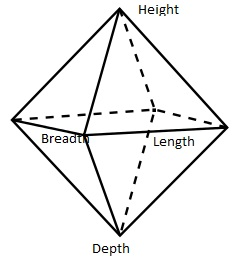
\includegraphics[scale=.5]{a20200913LengthBreadthHeightDepth-img001.jpg} 
 \caption{Quaternity}
 \end{wrapfigure}

\subparagraph{Length}
Length represents eternity, which has no end in place or time. It is God as Infinite, the source of all possibilities.

\subparagraph{Breadth}
\begin{quotex}
For thou lovest all things that are, and hatest none of the things which thou hast made. \flright{\textsc{Wisdom 11:25}}

Sun rises upon the good and the wicked, and rain falls upon the just and the unjust. \flright{\textsc{Matthew 5:45}}

\end{quotex}
Breadth is God's love, which has no boundaries. Breadth extends throughout the world process because God loves what He created.

\subparagraph{Height}
Height means that God is above all. This is God as the Absolute, as Power, omnipotence.

\subparagraph{Depth}
Depth signifies that God is within. As such, God is Wisdom, Intelligence, Judgment.

\paragraph{Contemplation}
\begin{quotex}
Discursive thought is satisfied when it arrives at a well-founded conclusion. Now, this conclusion is the point of departure for contemplation. It fathoms the profundity of this conclusion at which discursive thought arrives. Contemplation discovers a world within, which discursive thought simply verifies as ``true". \flright{\textsc{Valentin Tomberg}}

\end{quotex}
Knowing these attributes through reason is not the same as comprehension. To comprehend, one must first become holy. Then you will know from your own experience. \textbf{Holy love} and \textbf{holy fear} make a man holy. Fear responds to the height and depth; love to the length and breadth. Teachings, and there are many in our day, that neglect one or the other will not lead to comprehension; worse, they lead to incomprehension. Love without Fear is vapid; Fear without Love is heartless.

Love that includes perseverance and long-suffering is the length. Love extended to enemies is the breadth.

Fear of God's irresistible power is the height. Fear of God's wisdom and judgment is depth.

\begin{quotex}
But to us God hath revealed them, by this Spirit. For the Spirit searcheth all things, yea, the deep things of God. \flright{\textsc{1 Corinthians 2:10}}

\end{quotex}
To comprehend the deep things of God requires more than knowing the truth.

\begin{quotex}
[Contemplation] becomes active when it is a question of something deeper than the question: Is it true or false? It perceives more the \textbf{significance} of the truth discovered by discursive thought and also why this truth is true in itself, i.e. it reaches to the mystical or essential source of this truth. How does it arrive at this? By listening in silence. It is as if one wanted to recall something forgotten. \flright{\textsc{Valentin Tomberg}}

\end{quotex}
A fact penetrates the soul when it has meaning, otherwise its truth is irrelevant to life.

\begin{quotex}
Psychological truths are not metaphysical insights; they are habitual modes of thinking, feeling, and behaving which experience has proved appropriate and useful. So when I say that the impulses which we find in ourselves should be understood as the ``will of God," I wish to emphasize that they ought not to be regarded as an arbitrary wishing and willing, but as absolutes which one must learn how to handle correctly. \flright{\textsc{Carl Jung}, \emph{Aion}}

\end{quotex}
Thus, as Saint Bernard tells us, the revelation of length, breadth, height, and depth as true is incomplete. Jung explains why this is so psychologically:

\begin{quotex}
the psychic phenomenon cannot be grasped in its totality by the intellect, for it consists not only of \emph{meaning} but also of \emph{value}, and this depends on the intensity of the accompanying feeling-tones. 

\end{quotex}
Reason can describe the meaning of the quaternity, but holy love and fear are necessary to reveal its value. On the personal level, there are four attributes corresponding to the divine four:

\begin{itemize}
\item \textbf{Marvel} at the height of majesty 
\item \textbf{Fear} the abyss of judgment 
\item \textbf{Burn} with the fire of love 
\item \textbf{Endure} with perseverance 
\end{itemize}
Saint Bernard then describes four modes of contemplation associated with the dimensions of the quaternity.

\subparagraph{Wonder at Majesty}
The first and greatest is to wonder at the majesty of God. This demands a purified heart that is freed from vices and released from sin. Then it can ascend easily to heavenly things. Sometimes the contemplative can be rapt in amazement and ecstasy, even if only for a moment.

This is associated with height.

\subparagraph{Judgment of God}
The contemplation on God's judgment may strike fear to outsiders because it is indeed frightening. Yet it drives out vices, strengthens virtues, initiates into wisdom, protects humility. Humility is the foundation of virtue.

This is associated with depth.

\subparagraph{Remember Kindnesses}
Remember with gratitude the kindnesses and graces received from God. This is a reminder to love God always.

This is associated with width.

\subparagraph{Endurance}
\begin{quotex}
one thing I do, forgetting what lies behind and straining forward to what lies ahead \flright{\textsc{Phil 3:18}}

\end{quotex}
Forget what is past and contemplate the expectation of what is promised. This nourishes patience and promotes perseverance. What is promised is eternal.

This is associated with length.

\paragraph{The Beginning of the Search}
Saint Bernard recommends these contemplations to those seeking God. They don't need to be formal or structured or long. You can practice them at any time throughout the day. It might even take a moment, even a passing thought. At the very least, these contemplations are superior to long-winded discussion. As Saint Bernard concludes:

\begin{quotex}
God is sought more worthily and found more easily by prayer than by discussion. 

\end{quotex}


\textit{Acknowledgments:} Quotes from Saint Bernard are from the Paulist Press edition of the \emph{Selected Works of Saint Bernard of Clairvaux}.

Tomberg quotes are from \emph{Meditations on the Tarot}, Jung quotes from \emph{Aion}. (emphases are mine)

\flrightit{Posted on 2020-09-13 by Cologero }

\begin{center}* * *\end{center}

\begin{footnotesize}\begin{sffamily}



\texttt{Matt on 2020-09-22 at 00:23 said: }

You finally answered the question I asked 5 years ago in your post ``Innate Wisdom and Collective Initiation" (\url{https://www.gornahoor.net/?p=1721}). The question was, ``how does height differ from depth?" 5 years is a lengthy time, but it's not an eternity. I'll remember this kindness.


\end{sffamily}\end{footnotesize}
